%!TEX root = ../thesis.tex
\chapter{Applications \& Discussion}

This chapter presents a discussion of MapperGUI's software design and its consequences for musical mapping, as well as revisions made to the code since the initial release. The interface's features are explored in an attempt to evaluate the successes and failures of the design. Feedback from users was gathered throughout the project and through informal interviews after the software's release. This feedback is summarized and presented here. A modification to the code, motivated by feedback from users, is also described. MapperGUI is then compared to similar interfaces, analyzing especially for new features that could be incorporated into our flexible framework. Finally, the system is evaluated overall with respect to the project's initial goals.


%%%%%%%%%%%%%%%%%%%%%%%%%%%%%%%%%%%%%%%%%%%%%%%%%%%%%%%%%%%%%%%%%%%%%%%%%%%%%%%%%%%%%%%%%%%%%%%%%%%%%%%%%%%%%%%%%%%%%%%%%%%%%%%%%%%%%%%%%%%%%%%%%%%%%%%%%%%%%%%%%%%%%%%%%%%%%%%%%%%%%%%%%%%%%%%%%%%%%%%%%%%%%%%%%%%%%%%%%%%%%%%%%%%%%%%%%%%%%%%%%%%%%%%%%%%%%%%%%%
\section{User Feedback} % (fold)
\label{sec:user_feedback}

The entire MapperGUI project began with user feedback from prior GUIs for libmapper. Throughout the design process functional versions of MapperGUI were provided to libmapper users. Their feedback was crucially important to the evolution of the software. After the first official release of MapperGUI, long-term users were informally interviewed. These users were questioned specifically as to the projects with which utilized MapperGUI in an attempt to learn more concretely about the variety of use-cases for the software.

Even at this early stage of release, users have already incorporated MapperGUI into a wide variety of projects. This reflects our initial assumptions (based on experiences with prior GUIs) that a successful GUI must be flexible. Throughout development MapperGUI was used as an experimental tool and aid in designing DMIs. MapperGUI was used in concert with motion capture systems, vibro-tactile feedback and even loaded onto a Raspberry PI\footnote{TODO}. During this whole process users encountered problems, had ideas for extensions and used the GUI in ways we never would have imagined.



%for response to vibrotactile feedback in a motion-capture study. It was also used in a motion capture setting for the design of an interactive audio installation. In the latter situation MapperGUI was required to handle many signals per single device, as each person in the room required 25 three-dimensional markers (75 signals total). A DMI designer has been using MapperGUI to test mappings for her input device with a single sound synthesizer, each containing about 30 signals.

%MapperGUI is being used as a development tool as well. A programmer is attempting to build a software bridge between libmapper and the Arduino\footnote{TODO}. She uses MapperGUI to test the robustness and effectiveness of the software, and has even successfully loaded the GUI onto a raspberryPI\footnote{TODO}

\begin{table}
\begin{center}
\begin{tabular}{l p{5cm} p{5cm}}
	\hline\hline
	user&use case&concerns\\
	\hline
	Mailis&Intonespacio&saving and loading\\
	Hakon&Experimenting with vibrotactile feedback and motion capture systems&Switching between various mappings\\
	Clayton&An interactive space using motion capture&Reliability of network\\
	Julie&libmapper code for firmata&Speed of function (she's using a rasperry Pi)\\
	\hline
	Andrew Stuart&teaches class with libmapper&\\
	Gestes (Marlon)&Performance, etc.&Hide unconnected\\
\end{tabular}
\end{center}	
\end{table}

Hakon Knutzen, Mailis Rodrigues, Clayton Mamedes, Julie Ren\'e
		%Mailis, Clayton, Hakon, Julie


	\subsection{General feedback} % (fold)
	\label{sub:general_feedback}

Most of our users had used libmapper previously, and had attempted to compile and use the library from scratch. Many commented on how well MapperGUI lowered the barriers to entry for non-technical users. Users who had never used libmapper before pointed out how much time had been saved in their work flow, versus when they used to hard-code mappings.

The best reviewed feature of MapperGUI was definitely the linear scaling control of the top bar. For users who previously needed to detect signal minima and

Most users were very impressed by the auto-scaling feature of the
	
	% subsection other_feedback (end)

	\subsection{Saving \& loading} % (fold)
	\label{sub:saving_and_loading}

Nearly all users made use of the saving and loading features in some way. For both experimental and design-based setups, returning to prior mappings is very useful, as it avoids the tedium of performing the same tasks repeatedly.

We received criticism for the na\"ive loading system. One user found it tedious that mappings would accumulate when loading multiple. He required rapid switching between the same few mappings for his experiment. Once these mappings were created there was little that needed to be done to modify them. For the experiment it became tedious to erase a previous mapping before loading a new one. Obviously in a live-performance context the amount of delay that would be created with this kind of task would be unacceptable. 

Another user wished to switch between mappings in his work, but required some kind of intermediate space between the states. Ideally loading would have the option of blending between two mappings, such that the transition is not too harsh for the audience. To maintain this functionality, the actual saving and loading of patches was transferred to Max/MSP for this project.

In a situation with many devices of the same class, loading a single mapping can be somewhat absurd. Because each connection will be loaded $m*n$ times, where $m$ is the number of similarly named input devices, and $n$ is the number of relevant output devices, certain simple mappings can result in hundreds of unwanted connections when a mapping is loaded. Perhaps some kind of staging area wherein the user must explicitly for which devices he or she wishes to load a mapping could solve this problem.
	
	% subsection saving_&_loading (end)

	\subsection{Reliability \& Responsiveness} % (fold)
	\label{sub:reliability_and_responsiveness}

Multiple users commented on the frustrating nature of interacting with MapperGUI when it became out of sync with the libmapper network. 
	
	% subsection reliability_and_responsiveness (end)

	\subsection{Effectiveness of Alternate Views} % (fold)
	\label{sub:effectiveness_of_alternate_views}

GridView and HiveView have only recently been recently included into the program. As a result most of our users are much more familiar with ListView. 
	
	% subsection effectiveness_of_alternate_views (end)
	
% section user_feedback (end)

%%%%%%%%%%%%%%%%%%%%%%%%%%%%%%%%%%%%%%%%%%%%%%%%%%%%%%%%%%%%%%%%%%%%%%%%%%%%%%%%%%%%%%%%%%%%%%%%%%%%%%%%%%%%%%%%%%%%%%%%%%%%%%%%%%%%%%%%%%%%%%%%%%%%%%%%%%%%%%%%%%%%%%%%%%%%%%%%%%%%%%%%%%%%%%%%%%%%%%%%%%%%%%%%%%%%%%%%%%%%%%%%%%%%%%%%%%%%%%%%%%%%%%%%%%%%%%%%%%
\section{Testing program responsiveness} % (fold)
\label{sec:testing_program_responsiveness}

Extension of interface features discussed in section \ref{sec:extension_of_control_and_visual_elements} leads to some control possibilities that could be difficult for the GUI to handle. Addition of shortcut keys for connecting, linking, disconnecting and unlinking, as well as the ability to select multiple devices and signals at once allows users to create and delete hundreds of connections with a single keypress. Na\"{i}ve saving and loading produces to situations where dense mappings will accidentally be applied to several instruments at once.

Though the ``update display'' model works extremely well for code modularity, it generates awkward situations when dealing with massive network operations. Since the system updates the entire display with each change to the network, deleting 100 links (if the user is clearing a large network) results in 100 independent \url{delete_link} messages arriving at the monitor. For each one of these messages, the display will fully update. In the case of the list view mode, all arrows will be cleared, and redrawn with one fewer present (as if the links are being deleted one-by-one). In total 4950 arrow drawing operations\footnote{$99 + 98 + 97 + ... + 2 + 1 = \frac{99*100}{2}$. Note that $\frac{n*(n+1)}{2}$ arrows will be drawn for any $n$ number of connections or links.} will occur, resulting in siginificant delay. 

As reported by users in section \ref{sub:reliability_and_responsiveness}, any GUI operation that takes more than a few seconds, without some kind of visual feedback (like a ``loading'' bar), leads to frustration and mistrust of the program. Obviously, if the GUI is going to support these kinds of massive network manipulations, there needs to exist some way to keep them under control.

	\subsection{Rate limiting certain functions} % (fold)
	\label{sub:rate_limiting_certain_functions}

In order to prevent thousands of uneccesary, display re-draws, a ``waiting'' period was added to certain critical functions. This operating systems process is described in \shortciteN{os_concepts}. Essentially certain functions no longer execute in the code immediately once called, instead, a delay timer starts. If the function is called again during this delay, the delay timer simply restarts. The function is only executed once the delay timer finishes. This way, if a function is called 100 times simultaneously, it will only execute once after a short delay. Figure \ref{fig:waiting_period} shows the effect of the waiting period if the function is called a single time, and if it is called once during the delay.

\begin{figure}[ht]
	\centering
		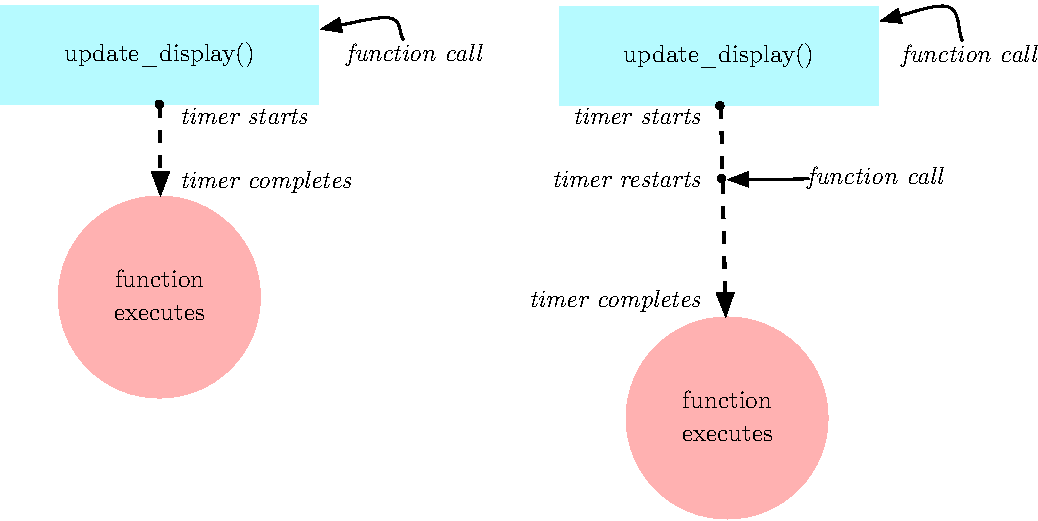
\includegraphics[width=1\textwidth]{figures/waiting_period}
		\caption{Illustration of a delayed function.}
		\label{fig:waiting_period}
\end{figure}

Two functions are limited in the GUI: \url{update_display} for all views and \url{update_arrows} for the list view. \url{update_display} is common to all views, and the massive network changes described above can result in many processor intesive functions to run needlessly. With the \url{update_arrows} function, operations that do not result in changes to the network (scrolling, changing tabs) require constant re-drawing.

Exactly how much time this delay should be set to is not obvious. If the delay is too short it is possible for massive network operations to still call the function many times if they arrive asynchronously. A too-long delay means that users may notice for simple actions, like scrolling with a single arrow (causing the srolling to appear jerky). Another consequence of a long delay is that a process which calls the delayed function at a reglar interval could continuously restart the delay. In this case the function will \emph{never} execute, a situation known as ``starvation'' \shortcite{os_concepts}.

%37 ms after brief testing
	
	% subsection rate_limiting_certain_functions (end)


% section testing_program_responsiveness (end)

%%%%%%%%%%%%%%%%%%%%%%%%%%%%%%%%%%%%%%%%%%%%%%%%%%%%%%%%%%%%%%%%%%%%%%%%%%%%%%%%%%%%%%%%%%%%%%%%%%%%%%%%%%%%%%%%%%%%%%%%%%%%%%%%%%%%%%%%%%%%%%%%%%%%%%%%%%%%%%%%%%%%%%%%%%%%%%%%%%%%%%%%%%%%%%%%%%%%%%%%%%%%%%%%%%%%%%%%%%%%%%%%%%%%%%%%%%%%%%%%%%%%%%%%%%%%%%%%%%
\section{Comparison to Similar Interfaces} % (fold)
\label{sec:comparison_to_similar_interfaces}

	\subsection{Junxion} % (fold)
	\label{sub:junxion}
		\cite{junxion}
	% subsection junxion (end)

	\subsection{Osculator} % (fold)
	\label{sub:osculator}
		\cite{osculator}
	% subsection osculator (end)

	\subsection{Other similar interfaces} % (fold)
	\label{sub:other_similar_interfaces}
	
	\begin{enumerate}
		\item Inclusive interconnections \shortcite{inclusiveinterconnections}
		\item Sense Stage \shortcite{senseStage}
		\item mpgcarepackage?
		\item Integra \shortcite{integra}
		\item Eaganmatrix: GRID VIEW! \shortcite{eaganmatrix}
		\item Patchage: a linking, dragging, connecting interface \shortcite{patchage}
	\end{enumerate}

	% subsection other_similar_interfaces (end)

% section comparison_to_similar_interfaces (end)

%%%%%%%%%%%%%%%%%%%%%%%%%%%%%%%%%%%%%%%%%%%%%%%%%%%%%%%%%%%%%%%%%%%%%%%%%%%%%%%%%%%%%%%%%%%%%%%%%%%%%%%%%%%%%%%%%%%%%%%%%%%%%%%%%%%%%%%%%%%%%%%%%%%%%%%%%%%%%%%%%%%%%%%%%%%%%%%%%%%%%%%%%%%%%%%%%%%%%%%%%%%%%%%%%%%%%%%%%%%%%%%%%%%%%%%%%%%%%%%%%%%%%%%%%%%%%%%%%%
\section{Evaluation of Goals} % (fold)
\label{sec:evaluation_of_goals}
	Are sections graphically unified? (Is this even necessary?)
	%Why is what what on the top bar`'

	%maybe write about different views here?

% section evaluation_of_goals (end)




